\documentclass[conference]{IEEEtran}


% Fonte em português brasileiro
\usepackage[american]{babel}
\usepackage[utf8]{inputenc}
\usepackage{enumerate}
\usepackage{setspace}
\usepackage{pgfgantt}
\usepackage{booktabs}
\usepackage{listings}
\usepackage{hyperref}
\usepackage{xspace}
\usepackage{balance}

% Default fixed font does not support bold face
\DeclareFixedFont{\ttb}{T1}{txtt}{bx}{n}{12} % for bold
\DeclareFixedFont{\ttm}{T1}{txtt}{m}{n}{12}  % for normal

% Custom colors
\definecolor{keywords}{rgb}{0.5,0,0.35}
\definecolor{comments}{RGB}{0,0,113}
\definecolor{red}{RGB}{160,0,0}
\definecolor{green}{RGB}{0,150,0}
 
\lstset{language=Python, 
        basicstyle=\ttfamily\small, 
        keywordstyle=\color{keywords}\bfseries,
        commentstyle=\color{comments},
        stringstyle=\color{red},
        showstringspaces=false,
        %identifierstyle=\color{red},
       }
       
% Identação e Margens
\usepackage{fullpage}      % Margens
\usepackage{indentfirst}   % Autoidentar

% Figuras
\usepackage{graphicx}       % Pictures

\title{Mining Android Sandox: Some possible improvement to be done ?}

\author{
\IEEEauthorblockN{
    Francisco Handrick da Costa\IEEEauthorrefmark{1},
    Ismael Medeiros\IEEEauthorrefmark{1},
    Rodrigo Bonif\'{a}cio\IEEEauthorrefmark{1},
    Marcio Ribeiro\IEEEauthorrefmark{3}, \\ 
    Gabriel Martins\IEEEauthorrefmark{1},
    Mira Mezini\IEEEauthorrefmark{2}, and
    Krishna Narasimhan\IEEEauthorrefmark{2}
}

\IEEEauthorblockA{
  \IEEEauthorrefmark{1}Computer Science Department, University of Bras\'{i}lia, Brazil,
  \IEEEauthorrefmark{2}Software Technology Group, TU Darmstadt, Germany, \\ 
  \IEEEauthorrefmark{3}Institute of Computing, Federal University of Alagoas, Brazil
  }
}


\newcommand{\droidxp}{DroidXP\xspace}

\begin{document}
\maketitle

\IEEEtitleabstractindextext{
\begin{abstract}
The widespread use of smartphones in our daily lives has elevated concerns regarding their security among researchers and practitioners.
Particularly, security issues are highly prevalent in Android, the most popular mobile operating system. Previous research has explored
various techniques to address these concerns, including the Mining Android Sandbox approach (\mas), which aims to identify malicious behavior in repackaged Android applications (apps).
However, earlier studies have been limited by small datasets, typically consisting of only \appsSmall pairs of original and repackaged apps.
This limitation raises questions about the external validity of their findings and whether the MAS approach is scalable to larger datasets.
To address these concerns, this paper presents the results of an experiment that replicates state-of-the-art research on evaluating the
accuracy of the \mas. Unlike previous studies, our research employs a dataset that is an order of magnitude larger, comprising \apps
pairs of apps covering a more diverse range of Android malware families. Surprisingly, our findings indicate a significant drop in the accuracy of the MAS approach for identifying malware, with
the \fone decreasing from \fscoreSmall in previous studies to \fscore in our larger dataset.
Upon closer examination, we discovered that the higher representation of malware from the gappusin family partially accounts for the increased
number of instances where the \mas fails to correctly classify a repackaged app as malware. Additionally, we investigated the impact of two extensions—--Trace Analysis and Parameter Analysis—implemented
from the literature to enhance the \mas. However, these extensions only marginally improved the approach's performance, with both extensions combined increasing accuracy by 8\%
(from 52\% to 60\%)—--still falling short of the accuracy reported in previous studies.
Our findings highlight the limitations of the MAS approach, particularly when scaled, and underscore the importance of complementing it with other techniques to effectively detect a
broader range of malware. This opens avenues for further discussion on addressing the blind spots
that affect the accuracy of the MAS approach.
\end{abstract}
}

%\begin{IEEEkeywords}
%  Android Malware Detection, Dynamic Analysis, Mining Android Sandboxes
%\end{IEEEkeywords}

\section{Introduction}\label{sec:introduction}

Mobile technologies like smartphones and tablets have become fundamental to the way we function as a society. Almost two-thirds of the world population
uses mobile technologies~\cite{Comscore,DBLP:journals/tse/MartinSJZH17}, with the
Android Platform dominating this market and accounting for more than 70\% of the \emph{mobile
market share} with almost 3.5 million Android applications~\footnote{In this paper, we will use the terms Android Applications, Android Apps, and Apps interchangeably, to refer to Android software applications} (apps)
available on the Google Play Store~\cite{Statista}. 
With increased popularity, comes increased risk of attacks---motivating efforts from both academia and industry to design and develop new techniques
to identify malicious behavior or vulnerable code in Android apps~\cite{10.1145/3017427}.


One of the most popular classes of malwares are based on repackaging apps~\cite{DBLP:conf/wcre/BaoLL18,le2018towards} where benign
versions of an app from an official app store are
%such as Google Play, 
infected with malicious code, e.g., to broadcast
sensitive information to a private server~\cite{DBLP:journals/tse/LiBK21}, and subsequently shared
with users using different app stores.  The focus of this paper is the Mining Android Sandbox, hereafter \mas, which has been shown effective
in detecting the popular class of Android malware based on 
repackaging benign apps. 
It  takes advantage of automated test case generation tools 
to explore the behavior of an app---in terms of calls to sensitive APIs---and then
generates a sandbox~\cite{DBLP:conf/icse/JamrozikSZ16}. During a normal
execution of the app, the sandbox might block calls to a sensitive API
that had not been observed during the exploratory phase. 


Previous studies~\cite{DBLP:conf/wcre/BaoLL18,DBLP:journals/jss/CostaMMSSBNR22} 
have compared the accuracy of  Android sandboxes for malware detection 
that were produced 
from 
%executing 
different test case generation tools, including Monkey~\cite{Monkey}, DroidBot~\cite{DBLP:conf/icse/LiYGC17}, and Droidmate~\cite{DBLP:conf/kbse/BorgesHZ18} tools.
The studies bring evidence that 
DroidBot outperforms the other test generation tools and leads to sandboxes that are more accurate in detecting malware with a classification rate of 70\%.
But these previous studies have two main limitations.
First, they use a small dataset of malware comprising only \appsSmall pairs of original/repackaged versions of an app. This decision
might compromise the external validity of previous studies. Second, their assessment do not investigate
the impact of repackaged characteristics on the accuracy of the \mas for malware classification, including
(a) whether or not the repackaged version is a malware, (b) the similarity between the original and the repackaged versions of an app,
and (c) the malware family (e.g., \fm{gappusin}, \fm{kuguo}, \fm{dowgin}, etc.) when the repackaged
version of an app is a malware.

%{\bf MM: The second part of the last sentence is not clear. Are similarity and malware family two different "malware characteristics"?}

%In this paper, we present the results of an investigation that aims to replicate previous studies~\cite{DBLP:conf/wcre/BaoLL18,DBLP:conf/scam/CostaMCMVBC20} in a larger dataset of app pairs (original/repackaged versions), and then explore whether a more diverse sample of app pairs has an influence on the accuracy of the \mas for malware identification. To this end, we explore the performance of the \mas using a larger dataset we curated for this research and DroidBot~\cite{DBLP:conf/icse/LiYGC17} as test case generation---the tool that, according to the literature, leads to the most accuracy Android sandbox. Our new dataset is an order of magnitude larger (it contains \apps pairs of original/repackaged apps), comprises a much more diverse similarity index, and covers a broader range of malware families. 

To empirically study the impact of these limitations on the reported results, in this paper we reconsider the performance of the \mas based on
DroidBot~\cite{DBLP:conf/icse/LiYGC17}---as we mentioned, the test case generation tool that, according to the literature, leads to the most accurate Android sandbox. 
Compared to previous studies~\cite{DBLP:conf/wcre/BaoLL18,DBLP:conf/scam/CostaMCMVBC20},
we use a curated dataset of app pairs (original/repackaged versions) that is, in terms of magnitude, larger than the previously used
dataset (it contains \apps pairs of original/repackaged apps).
 
{\bf Negative results.} Our study reveals a significantly lower
%on a larger and more diverse dataset (compared to previous studies), 
accuracy ($F_1$ score) of the \mas in comparison to what has been reported before (\fscore versus \fscoreSmall). 
An accuracy of \fscore is clearly unsatisfactory for a trustworthy malware classification technique.
This result motivated us to conduct a series of experiments 
to understand the reasons for the lower accuracy in our larger dataset, \textcolor{blue}{and a possible solution to revert it.}
%The original approach classifies an app as malware whenever there exists a difference between the sets of calls to sensitive APIs collected when running the test case generation tool over the original and repackaged versions of the same app.
First, we check the impact of the similarity between original and repackaged versions of
an app on the performance of the \mas for malware classification. Our results reveal a non significant association association between similarity and the accuracy of the \mas. 
%\kn{Saying there is no association is not the same as saying that similarity does not impact the accuracy. Somehow I feel this statement is very strong. I would rather say that we did not find any significant association between similarity and the accuracy of the \mas.
Second, we explore if the
malware family could explain the lower performance of the \mas for malware classification in 
our dataset.

Considering this second analysis, our results reveal that the \mas fails to correctly classify most of the samples from
the \gps malware family (a particular class of adware that frequently appears in repackaged apps). 
Out of the total of \appsGps samples within this family in our large dataset, the \mas failed to correctly classify \appsGpsFN samples as malware (false negative).
Our results reveal that this particular family is responsible for substantially reducing the recall of the \mas.
Our findings have two main implications, which open the discussion (a) on one important feature found at \gps malware family that should be
considered when building malware detection approaches that mine sandboxes, and (b) on the need to have a representative dataset, that should be labeled with sought
answers and which should leads close to real-life scenarios.
  

%{\bf MM: How is the last sentence different from the one preceding it? It appears to repeat what was just said, IMHO. Also, given that we highlight two distinguishing characteristics of the larger dataset -- similarity of apps and different malware -- I was expecting that we analyse the impact of both the diversity of apps and malware. But we report only that one particular kind of malware is responsible. The dissimilarity of app pairs has no effect? What about other families of malware?}
%

%{\bf MM: I don't get the logical implication that "Still" suggests. Also, (a) and (b) appear out of nowhere... how do they relate to what has been said before in the paragraph? What is blindspot that you are talking about here? How resp. from where do you derive the need to investigate further sources of information?}

The remainder of this paper is organized as follows. 
We provide background information on the \mas and the \mas for malware detection in
Section~\ref{sec:background}. Section~\ref{sec:experimentalSetup}
characterizes our experiments in terms of research goal, questions, metrics, datasets, and our procedures for data collection and data analysis. \textcolor{blue}{Section~\ref{sec:results}, Section~\ref{sec:resultsTraceParameter} and Section~\ref{sec:discussion} present the main findings of our experiments, results of others techniques that can complement the \mas, and possible threats to the validity of our results.} Finally,
Section~\ref{sec:conclusions} presents concluding remarks and possible future
work. The main artifacts we produced during this research are available in the
paper repository.

\begin{small}
  \begin{center}
    \url{https://anonymous.4open.science/r/paper-droidxptrace-results-F55A/}
  \end{center}
\end{small}

\section{Background and Related Work}\label{sec:background}

%% In this section, we introduce the concepts and terminology that are necessary to understand the reminder of this paper. First, Section~\ref{sec:sand} introduces some background information about \emph{sandboxes} within the security context. Section~\ref{sec:repackage} presents background information about repackaged application and how they introduce malicious behavior.
%% Finally, in Section~\ref{sec:android-sandbox} we review the \emph{mining sandbox approach} for detecting repackaged Android apps.

The Android bytecode language~\cite{DBLP:conf/issta/WangGMC15} favors reverse engineering tasks. That is, software developers can easily reverse-engineer real apps (benign), modify their contents by inserting malicious code (malware), repackage them with the malicious payloads, and re-publish them in app stores, including the Google Play Store. Repackaged Android apps can leverage the popularity of real apps, to increase its propagation and spread malware.  
Repackaging has been raised as a noteworthy security concern in Android ecosystem by stakeholders in the app development industry and researchers. Indeed, there are reports claiming that about 25\% of Google Play Store app content correspond to repackaged apps~\cite{DBLP:conf/sigmetrics/ViennotGN14}. Nevertheless, all the workload to detect and remove malware from markets by the stores (official and non-official ones), have not been accurate enough to address the problem. As a result, repackaged Android apps threaten security and privacy of unsuspicious Android app users, beyond compromising the copyright of the original developer~\cite{DBLP:journals/access/KimLCP19}. Aiming at
mitigating this threat, several techniques based on both static and dynamic analysis of Android apps have been proposed.


\subsection{Mining Android Sandboxes}\label{sec:android-sandbox}

A \emph{sandbox}
is a well-known mechanism to secure a system and forbid a software component from accessing
resources without appropriate permissions. Sandboxes have also been used to build an isolated
environment within which applications cannot affect other programs, the network, or other device data~\cite{DBLP:journals/peerj-cs/MaassSCS16}. The idea of using sandboxes emerged from the
need to test unsafe software, possible malware, without worrying about the integrity of the
device under test~\cite{DBLP:conf/esorics/BordoniCS17}, shielding the operating system from security issues.
To this end, a sandbox environment should have the minimum requirements to run the
program (make sure the program will not spill out of the sandbox), and make sure it will never
assign the program greater privileges than it should have, respecting the principle of
\emph{least privilege}. This principle ensures unauthorized access to resources,
improving the system's overall health. Within the Android ecosystem, sandbox approaches ensure the principle
of the \emph{least privilege} is ensured by preventing apps from having direct access to resources or data from other apps. Access to sensitives resources
like contacts list is granted through specific APIs (Application Programming Interface),
which are managed by permissions system~\cite{DBLP:journals/corr/abs-2109-06613}. 

%% The main market source for Android apps is Google Play Store. Unfortunately, it has
%% a flexible policy regarding the process of publishing apps, and therefore, many Android apps are removed from the
%% store because of issues related to malware\cite{DBLP:conf/msr/WangLL0X18}. Google Play tries
%% to minimize unauthorized access to sensitive resources by malicious apps,
%% listing each app with its requested permission. {\color{red}Those permissions are presented to Android
%% users at app installation moment since version 6}. However, some works presented that most users are careless regarding these permissions since they are only interested to run the app~\cite{DBLP:conf/soups/FeltHEHCW12}. This represents a great security breach since malware usually asks for more permissions than their APIs normally would require~\cite{DBLP:conf/ccs/FeltCHSW11}.

\begin{figure}[ht]
\centering
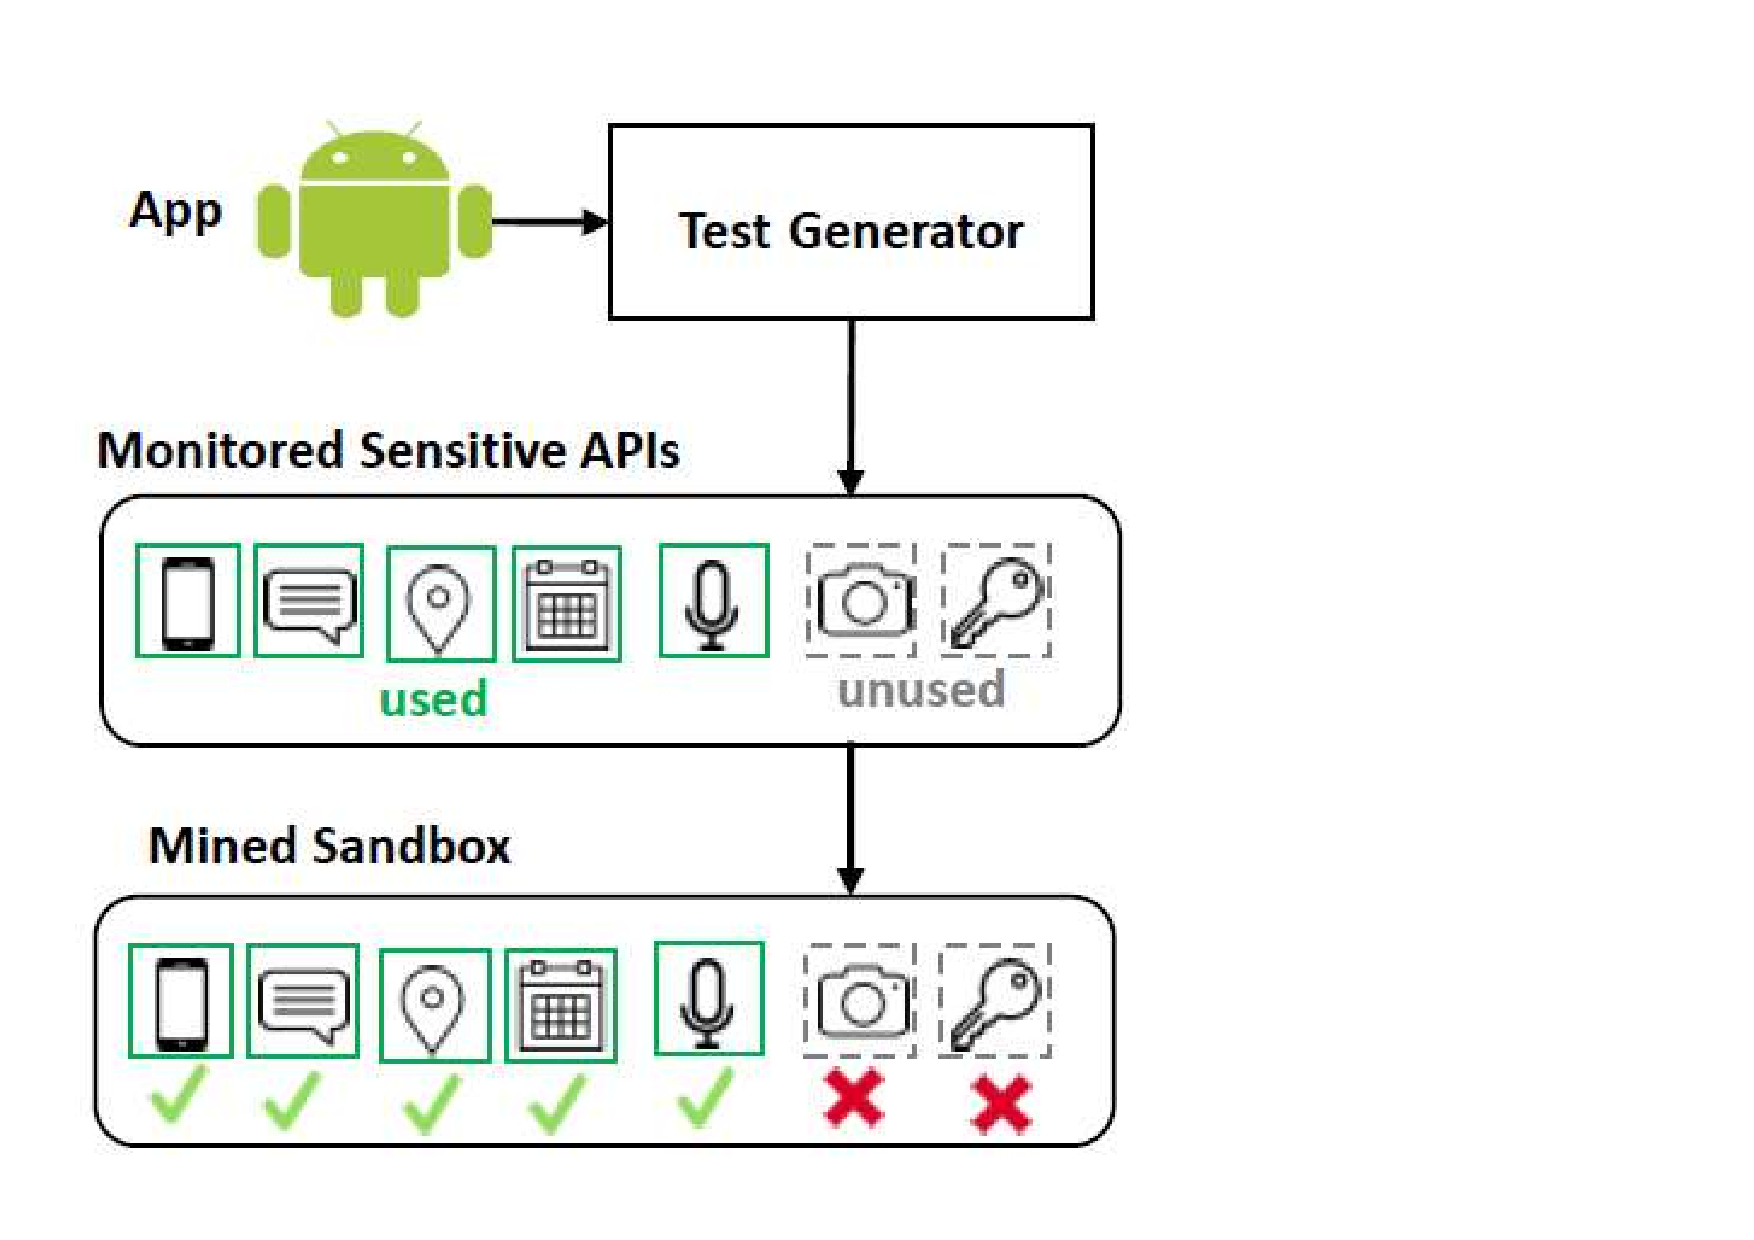
\includegraphics[scale=0.35]{images/mineSandbox.pdf}
\caption{Mine Sandbox.}
 \label{fig:mineSandbox}
\end{figure}

The Mining Android Sandbox approach~\cite{DBLP:conf/icse/JamrozikSZ16} (hereafter \mas) aims at automatically
building a sandbox through dynamic analysis (i.e., using automatic test generation tools).
The main idea is to explore apps based on their calls to sensitive APIs.
Thus, sandboxes build upon these calls to create safety rules and then block future
calls to other sensitive resources, which diverge from those found in the first exploratory
phase. Using a test generation tool named Droidmate~\cite{DBLP:conf/icse/JamrozikZ16},
Jamrozik et al.~\cite{DBLP:conf/icse/JamrozikSZ16} proposed a full fledged
implementation of the \mas, named Boxmate. 
Boxmate records the occurrences of calls to sensitive APIs and the UI events that triggers these calls,
like a button click. It is possible to configure Boxmate to record events associated with each sensitive call as
tuples (event, API), instead of recording just the set of calls to sensitive APIs. Jamrozik et al. argue that, in this way, Boxmate generates finer granularity results which
might reduce false alarms, even with the presence of reflection which is quite commonly used in
malicious apps~\cite{DBLP:conf/issta/0029BOK16}.

In fact, the \mas can be implemented using
a mix of static and dynamic analysis. In the first phase, one
can instrument an Android app to log any call to the Android sensitive methods.
After that, one can execute a test case generation tool (such as DroidBot
or Monkey) to explore the app behavior at runtime,
while the calls to sensitive APIs are recorded.
Figure~\ref{fig:mineSandbox} presents this general approach for \mas. This set of calls to sensitive APIs is then used
to configure the sandbox. 

%\todo[inline]{Since this figure is not discussed in the paper, we can remove it without any problem. I have enriched the previous paragraph, though, to make it
%  more necessary. Nonetheless, I will change this figure a bit, in order to
%represent the instrumentation phase.}



\subsection{Mining Android Sandbox for Malware Identification}

Besides being used to generate Android Sandboxes, the \mas is also effective 
to detect Android apps with suspicious behaviors~\cite{DBLP:conf/wcre/BaoLL18}. In this scenario, the \emph{effectiveness} of the approach
is estimated in terms of accuracy in which repackaged apps are identified.
The general mining sandbox approach (see Figure~\ref{fig:mineSandbox}) suggests
that the more efficient the test generator tool (for instance, in terms of code coverage),
the more accurate would be the resulting sandbox.


Figure~\ref{fig:sensitiveAPI} illustrates the \mas for
repackaged apps identification. We leverage DroidXP~\cite{DBLP:conf/scam/CostaMCMVBC20} to collect the set of sensitive APIs the versions of the apps call (benign/malign versions). As a first step, given one benign app version,
our approach first collects all calls to sensitive APIs from the app code through static analysis. Then, during the execution step,
we use dynamic analysis to collect all calls to sensitive APIs during the DroidBot test case execution. We configure DroidXP to execute DroidBot for a
period of $3$ minutes. Since some malicious app may use dynamic features (such as reflection) to introduce malicious behavior, which can change the behavior of the apps at runtime~\cite{DBLP:journals/spe/ZhangLTX18,DBLP:journals/tosem/LiTX19}, this second analysis is also important to disclose some sensitive APIs calls ignored by static analysis.

While our static analysis is made once, we execute dynamic analysis $3$ times. The result of static analysis and all executions is finally joined, forming a final set that contains all identified calls to sensitive APIs coming from the benign version of the app, as described at Figure~\ref{fig:sensitiveAPI}: ($S_{A}$, $D_{A1}$, $D_{A2}$, $D_{A3}$). We carry out the same procedure for the malicious version of the apps,
creating a distinct set of calls to sensitive APIs (now coming from the malicious version of the apps). In
a final step, we compare the two sets of calls to sensitive APIs ($Set_B, Set_M$). We use the following rules to
check for a malicious behavior. 

\begin{enumerate}
    \item If the difference between the two final sets is an empty set, we cannot distinguish the benign from the malicious version of the app (false negative).
    \item Otherwise, we successfully distinguish the benign from the malicious version of the app (true positive). 
    %\kn{Cant we replace the first part of the second point simply as "Otherwise" or is there some specific corner cases that I am missing}
\end{enumerate}

In addition, this procedure also enables us to identify the calls to sensitive APIs that are more frequently injected by the malicious version of the apps
in our dataset. 

%\fh{here I have to insert the figure}

\begin{figure}[ht]
\centering
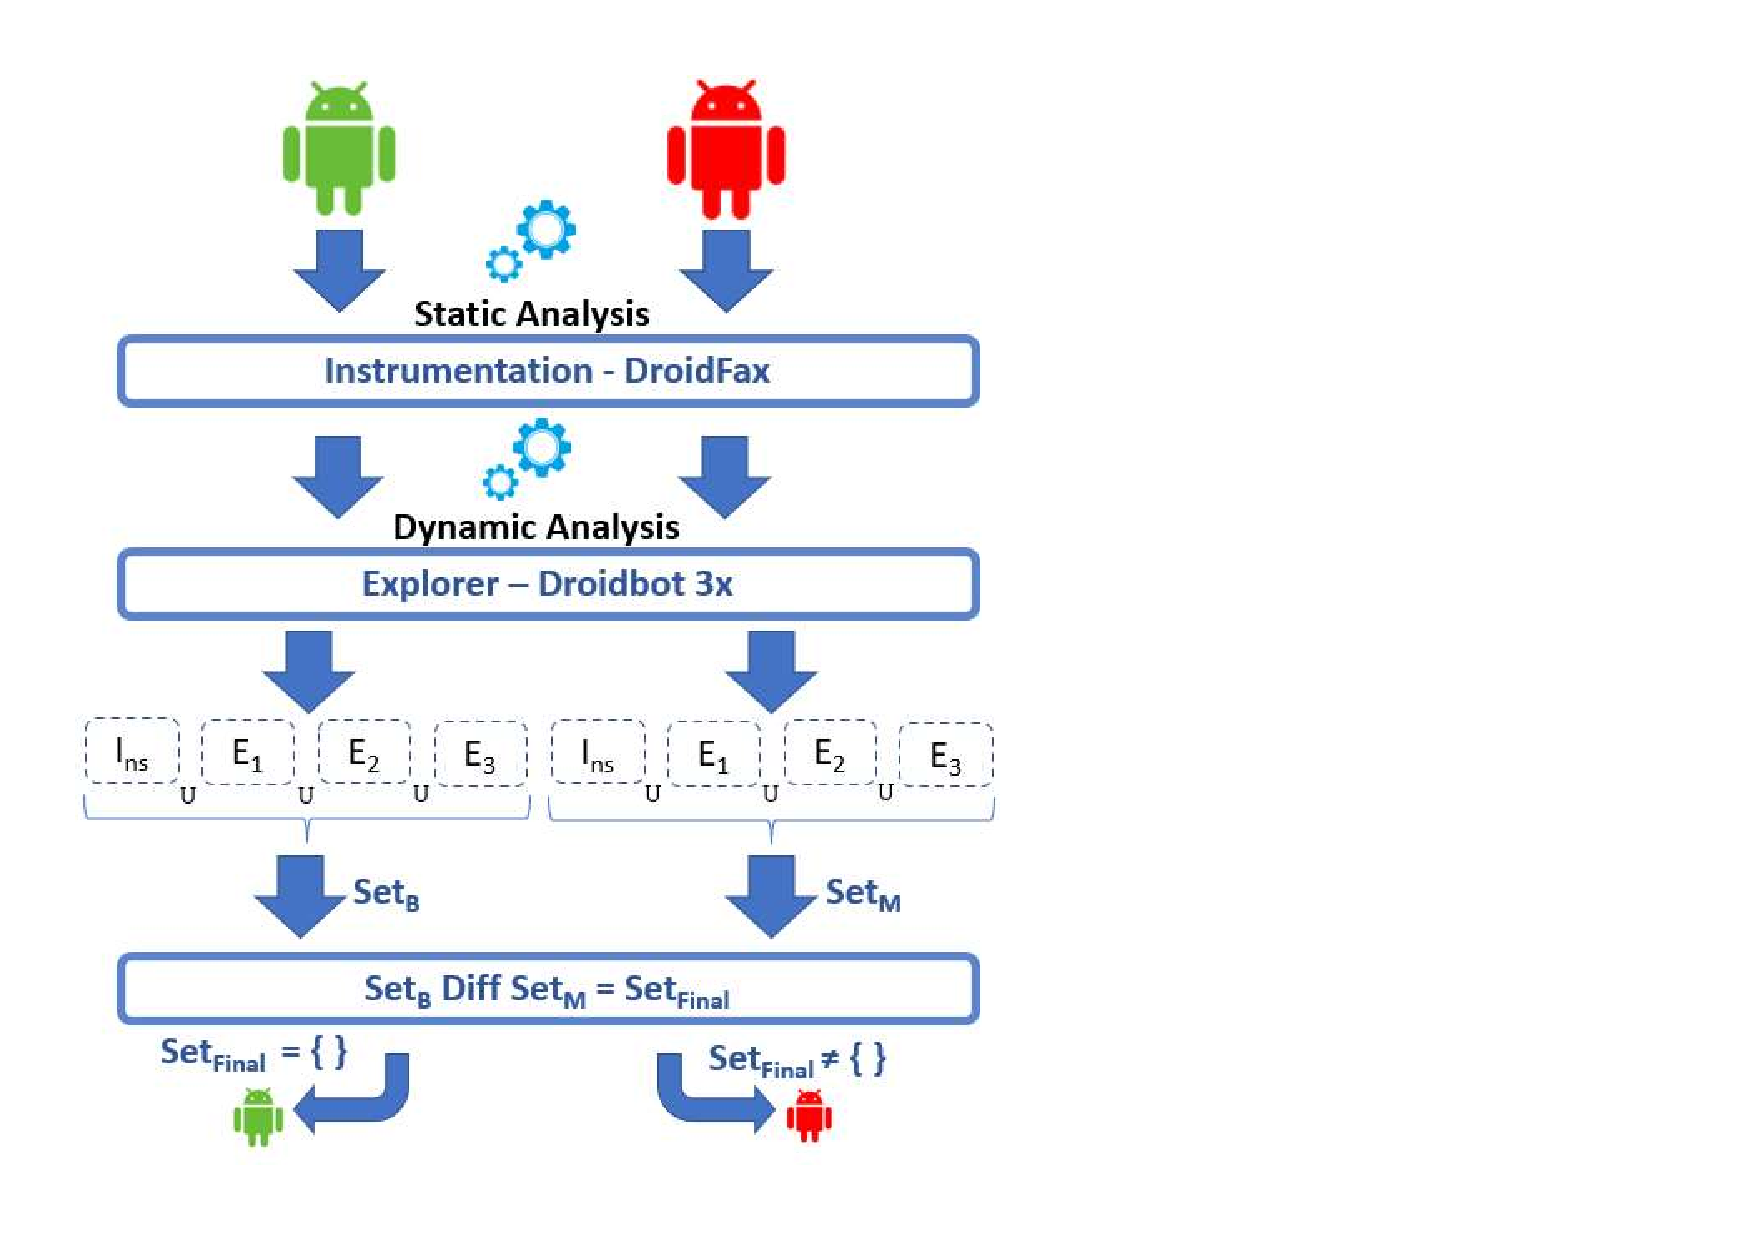
\includegraphics[scale=0.45]{images/sensitiveAPIdiff.pdf}
\caption{All procedure for suspicious app identification using sensitive API set diff.}
 \label{fig:sensitiveAPI}
\end{figure}



%\kn{I have commented out the subsection here as it seems redundant with the previous subsection}
%\subsection{The Mining Android Sandbox Approach for Malware Identification}

%The focus of our paper is in approaches that mine android sandboxes to classify Android Malware.
%There is a vast body of research in this direction. 

Costa et al. and and Bao et al.~\cite{DBLP:conf/wcre/BaoLL18,DBLP:conf/scam/CostaMCMVBC20} conducted empirical studies to investigate the effectiveness of \mas, exploring test generation tools, including DroidBot. Bao et al. found that, in general, the sandboxes constructed using test generators can detect more than $66$\% malicious apps in a dataset comprising $102$ pairs (benign/malicious). The study also presented that among $5$ test generation tools used, DroidBot~\cite{DBLP:conf/icse/LiYGC17} is the most effective sandbox.
Le et al.~\cite{le2018towards} extend the work of Bao et al. by combining more categories of sensitive APIs, and also considering the impact of actual parameters, combining sensitive APIs calls and input parameters of these APIs.
%\kn{What arguments? function parameters?}. 
Costa et al.\cite{DBLP:journals/jss/CostaMMSSBNR22} investigated the impact of static analysis to complement the accuracy of dynamic analysis tools for \mas. The study found that DroidFax~\cite{DBLP:conf/icsm/CaiR17a}, the static analysis infrastructure used in~\cite{DBLP:conf/wcre/BaoLL18}, is able to detect almost half of repackaged apps in a
dataset of $96$ pairs of benign/malicious apps.

%\todo[inline]{I could not understand why we did not cite our JSS work here}
%However, none of the aforementioned studies
% ~\cite{DBLP:conf/icse/JamrozikSZ16,DBLP:conf/wcre/BaoLL18,le2018towards}
%neither characterize the APIs included on the repackage versions nor investigate the
%possibility that trace analysis using call graph or analysis of
% the manifest file could complement the mining sandbox approach for malware identification.

\subsection{Extending the Mining Sandbox with Trace Analysis}

Our work, although closely related to previous studies, differs from them in several aspects.  First, our assessment is more comprehensive: instead of considering $102$ pairs of benign/malign apps, we execute our study considering \apps pairs of apps. Curiously, the performance of the \mas in our large dataset drops significantly. We then investigate which characteristics of the malware samples in the large dataset explain the lower performance. We observed and also explore an extension to the \mas that compare the traces from the app entry points to the calls to sensitive APIs, considering the benign and malign versions of the apps. 

As we discussed in the previous section, we build the dynamic call graphs that characterize the execution of each version of the apps in our dataset. Our goal
here is to explore how many pairs of apps call the same set of sensitive APIs, though using different call
traces. We hypothesize that differences in the traces might be used to complement the \mas for suspicious app identification. As such, here we execute the trace analysis for all app pairs of our dataset, and check if there are situations in which the basic version of the \mas was not able to correctly classify the malign version of an app as a piggybacked, however it has a different execution trace. For detecting different trace, we performed an evaluation of the dynamic call graph of each pair. Our procedure checks if there is some new node, representing a new sensitive API at malicious version, or a new edge($x$, $y$), where $x$ and $y$ indicates a method $x$ calling a sensitive method $y$.

%\rb{(Not sure if this is the right decision. I do not see any problem in running
%  this study for all pairs.)}. 
%% we  investigate those app pairs that were not described as a malware during the exploratory step, i.e,
%% the test generation tool DroidBot collected the same set of sensitive APIs for both version. If a dynamic call graph
%% of these app pairs presented different traces from entry point to sensitive APIs call at both versions, we suspect this to indicate presence of malware.
Figure~\ref{fig:callGraph} illustrates an example of benign and malicious call graphs.
At this example, although both app versions access the same set of sensitive resources, the
malicious version follows a different execution trace. 


\begin{figure}[ht]
\centering
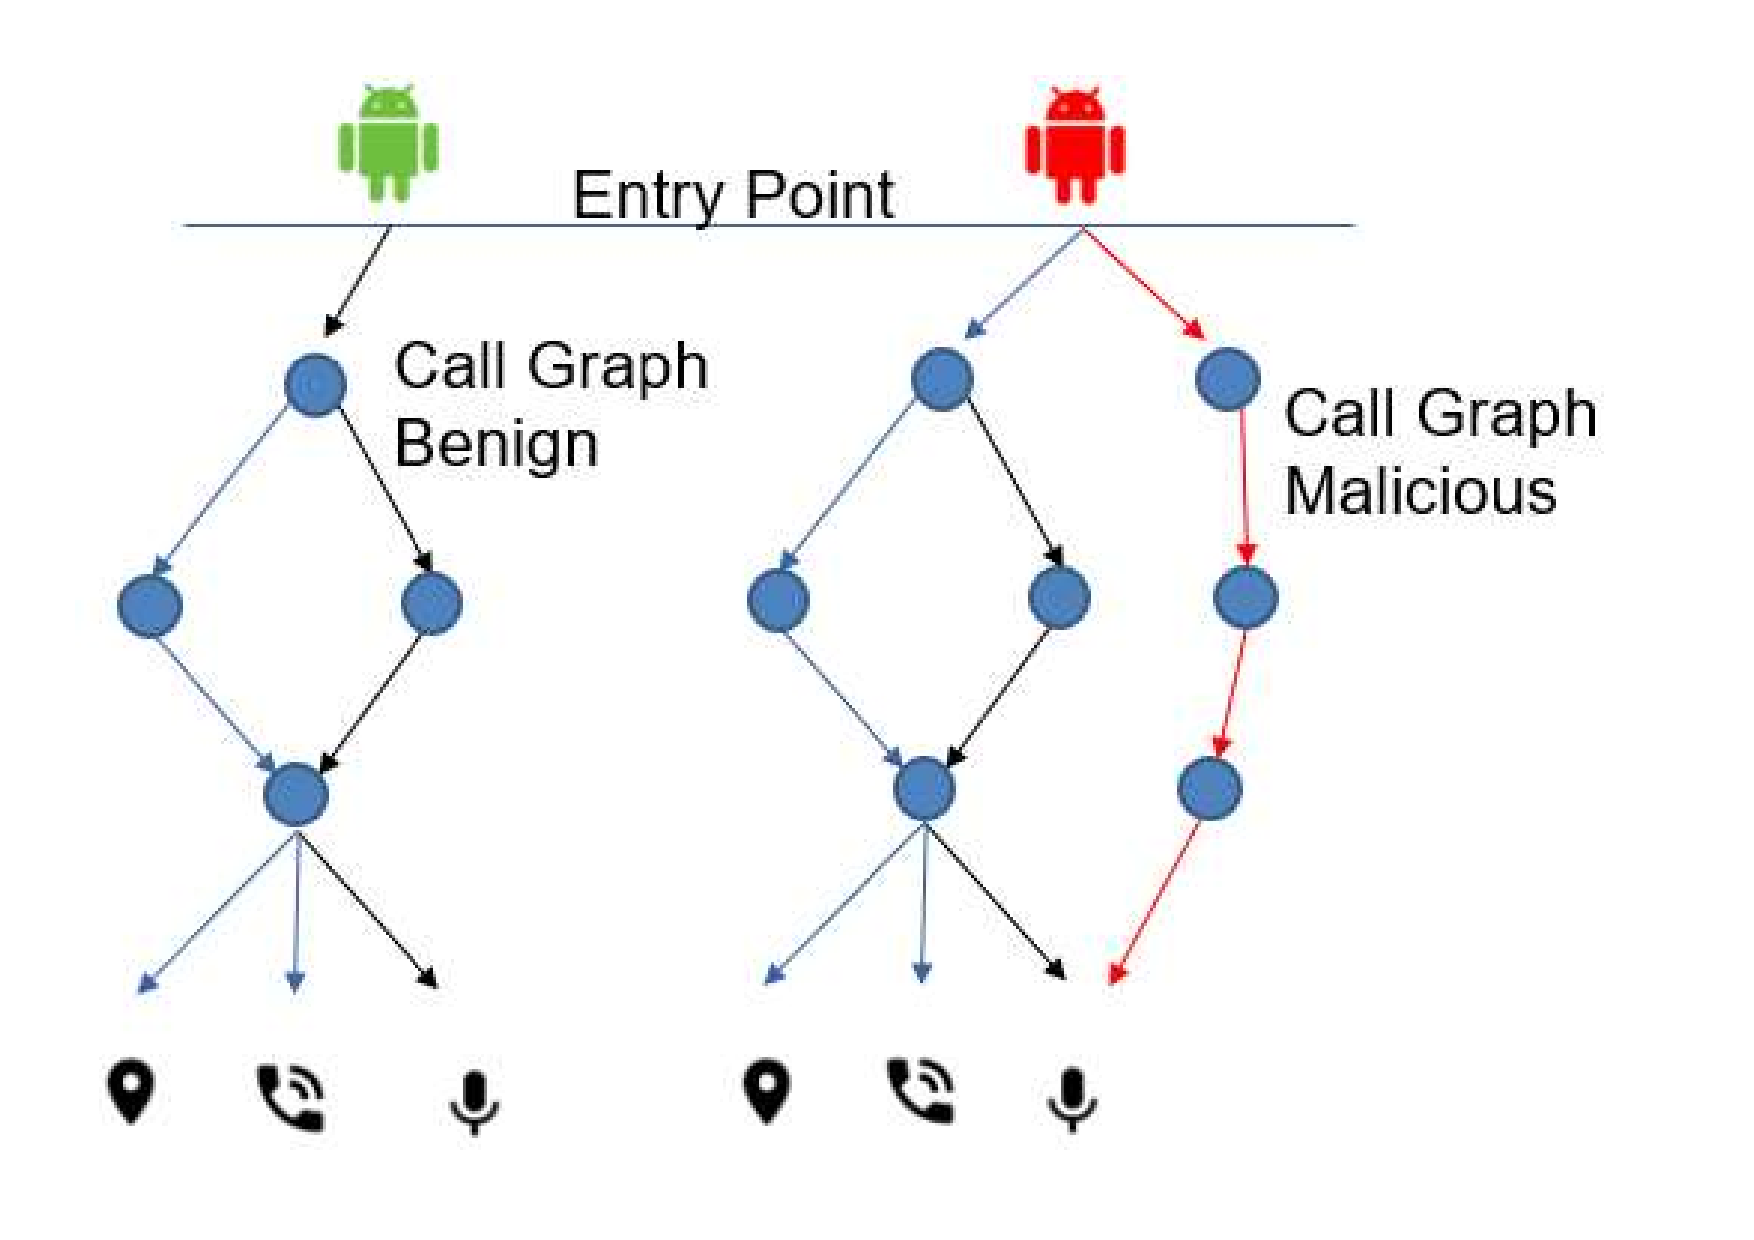
\includegraphics[scale=0.30]{images/maliciousCallGraph.pdf}
\caption{Illustrative example of the trace analysis. In this case, both versions call the same set of sensitive APIs. Nonetheless,
the traces between the entry point and the calls to sensitive APIs diverge.}
 \label{fig:callGraph}
\end{figure}


Figure~\ref{fig:maliciousTrace} shows an example of a trace injected in the malicious version of the
app \textbf{[com.android.remotecontrolppt]}. Here, the benign and malicious app versions access the same
sensitive method, \textit{getSubscriberid()}. This sensitive method returns the device's unique
subscriber ID, and requires the manifest file permission \texttt{READ\_PHONE\_STATE}, present in both app versions.
The original app accesses this method through two distinct traces (Trace 01 and Trace 02), which suggests an expected action from app user. However,
instead of the two original traces, the malicious version injected a third trace (Trace 03) containing as entry point a method that performs a stealth
computation on a background thread, \textit{doInBackground}, suggesting an action without user's awareness.


\begin{figure}
\centering
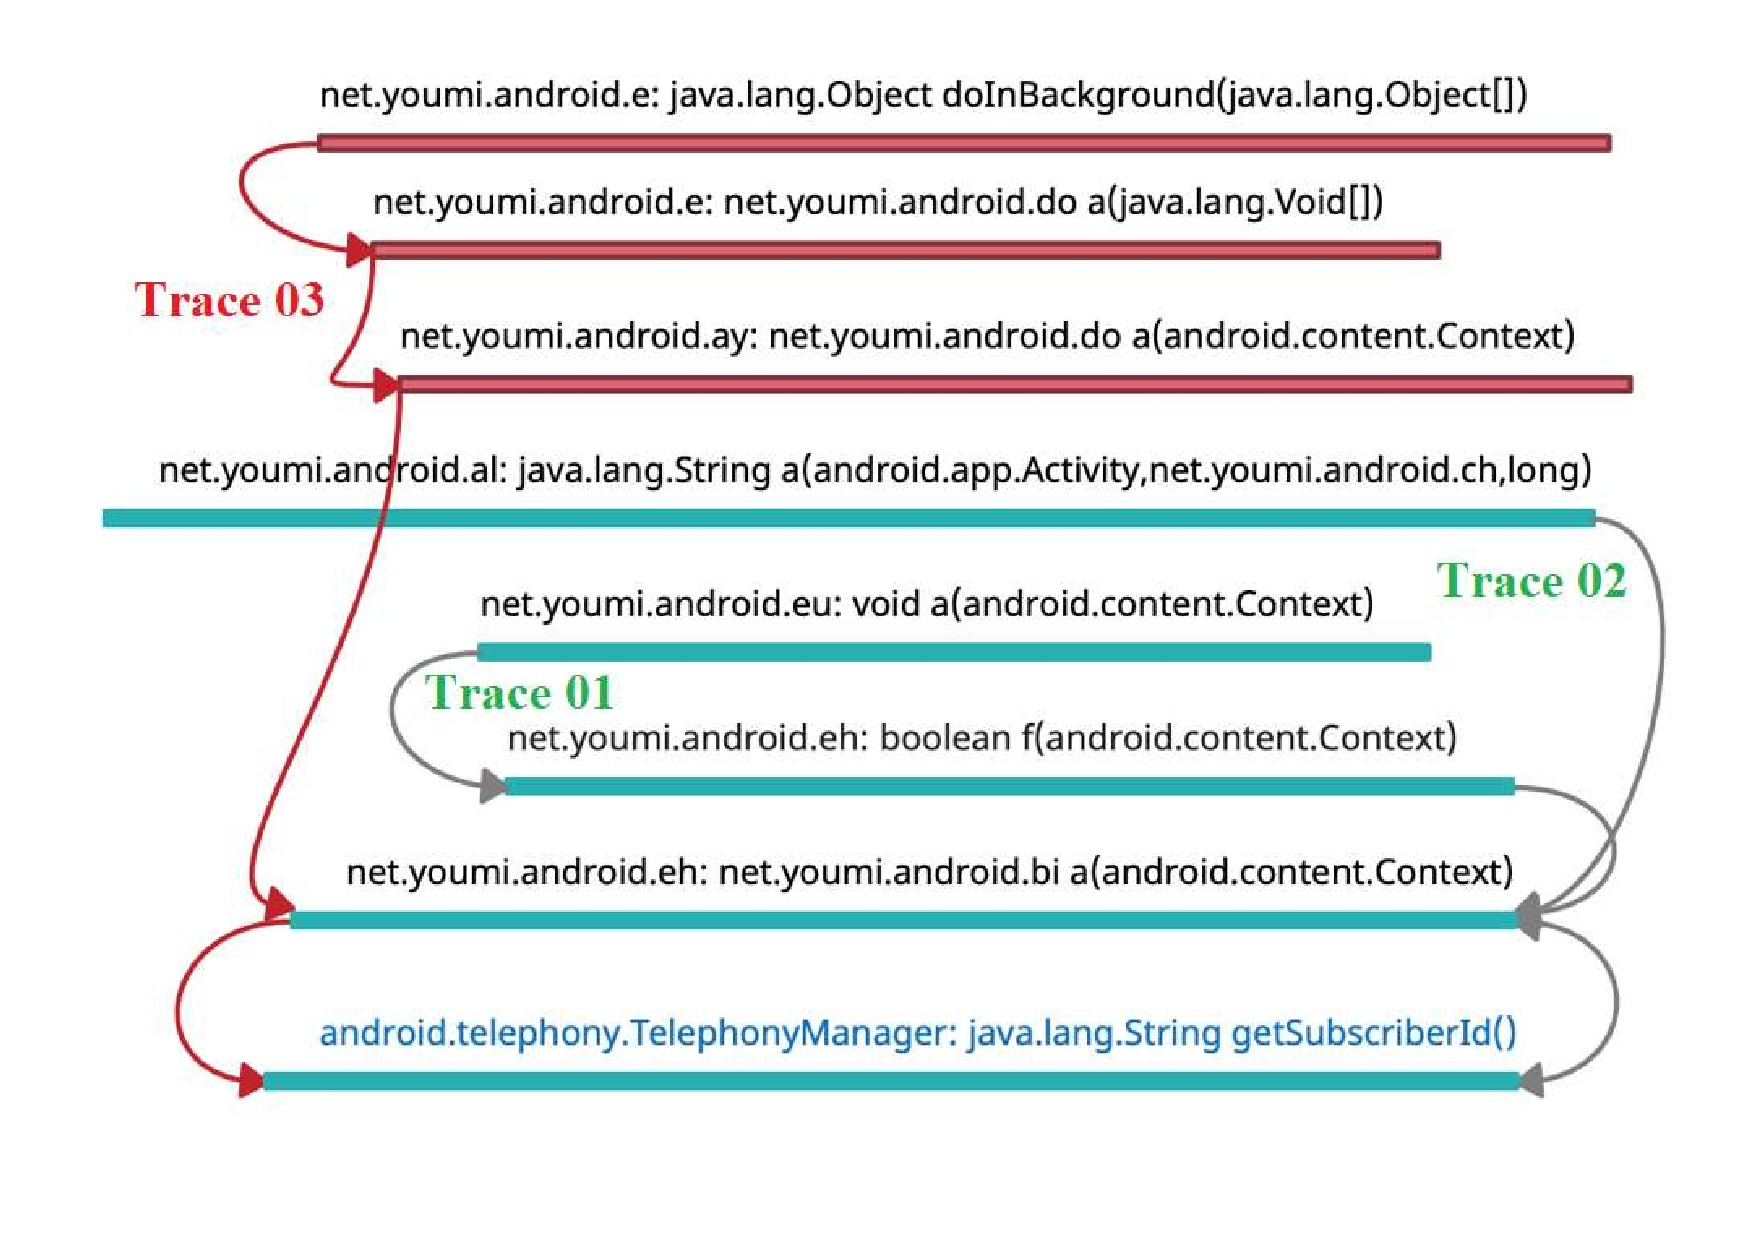
\includegraphics[scale=0.28]{images/maliciousTrace_example01.pdf}
\caption{Example of Malicious Trace.}
 \label{fig:maliciousTrace}
\end{figure}

\section{Sandbox Solution and its Weakness}\label{sec:sandbox}
\section{Methodology}\label{sec:methodology}
\section{Evaluation}\label{sec:evaluation}
\section{Related Work}\label{sec:relatedwork}
In this section, we discuss prior studies in two areas: Dynamic and Static Analysis on Android and mine Sandbox.

\subsection{Dynamic and Static Analysis on Android}\label{sec:analysis}

Dynamic and Static Analysis on Android Apps are important practices for developing security apps. There is a large body of work on both analysis for Android apps security. 

Several approaches for malware detection, based on sensitive methods call and permission control Android apps~\cite{DBLP:conf/mobicom/WeiGNF12,DBLP:conf/asiajcis/WuMWLW12,DBLP:conf/sp/LiDLDG21}. Cai et al.~\cite{DBLP:journals/tse/CaiR21} presented a longitudinal study on Android apps focusing on run-time behaviors. However, this work does not explore specifically on malware detection, since only benign apps were considered in their study, and just presented possible security gaps. Fangfang et al.~\cite{DBLP:conf/wisec/ZhangHZW014} proposed ViewDroid, which models the UIs (user interface) of Android apps as a directed graph. ViewDroid identify apps repackaging, comparing graphs structures in app pairs (benign/malicious).

Through static analysis on Android Manifest files, Kim et al. proposed RomaDroid~\cite{DBLP:journals/access/KimLCP19}, a repackage Android app detector based on Manifest file. They proposed that Manifest file apps could be represented as a tree-based structure and also by a single string from this structure. Hence, RomaDroid compares the strings of the benign and malicious app, using the longest common subsequence algorithm (LCS). Au el al.~\cite{DBLP:conf/ccs/AuZHL12} also used static analysis on Android Manifest files to detect vulnerabilities in Android apps. They mapped Android APIs sensitive calls and your respective required permissions.

A relevant prior work ~\cite{DBLP:journals/tifs/0029LBKTLC17} done by Li et al. provided a systematized knowledge
on Android app security to the community. They conducted an empirical study comparing malicious repackage app with their benign counterparts (1,497 app pairs). They found that the majority of Android malware are nothing but repackaged versions of benign apps, that are done with no sophisticated way, many times automatically and using library code.

There are other works that focus on comparison of app code, and try to check similarity to detect repackaged apps. Following this approach, Crussell et al.~\cite{DBLP:conf/esorics/CrussellGC12} proposed  DNADroid, which compares program dependence graphs, and Zhou et al.~\cite{DBLP:conf/codaspy/ZhouZJN12} DroidMoss which detect and analyze repackaged apps adopting a fuzzy hashing technique.

\subsection{Mine Sandbox}\label{sec:mineSandbox}

The technique called mine sandbox consists of explores software behavior by means of automatic test generation tools and, thus, prevent
Android apps from suspicious behaviors. Using a test generation tool named Droidmate~\cite{DBLP:conf/icse/JamrozikZ16}, Jamrozik et al.~\cite{DBLP:conf/icse/JamrozikSZ16} proposed an approach called Boxmate, the first mine Sandbox approach for Android environment. Boxmate records the occurrences of calls to sensitive APIs and input parameters. They found that Boxmate has low false alarm rate when checking Boxmate against 18 benign app that uses reflection API (\textit{java.util.reflect}) package. The reflection API at runtime can modify behavior of classes, interfaces and methods, and it is quite commonly used at malicious app~\cite{DBLP:conf/issta/0029BOK16}. Jamrozik et al. did not consider real malware to validate their approach, beyond they used a small sample of Android apps.

Bao et al.~\cite{DBLP:conf/wcre/BaoLL18} conducted an empirical study to investigate the effectiveness of mine sandboxes, exploring test generation tools, including Droidmate. The authors found that in general, the sandboxes constructed by test generator tools can detect more than $70$\% malicious apps in a dataset comprising $102$ pairs (benign/malicious). The study also presented that among 5 test generate tools used, DroidBot~\cite{DBLP:conf/icse/LiYGC17} constructed the sandbox more efficient to detect malware.

However, Bao et al. do not investigate the effectiveness of mine sandboxes considering parameter values in the called APIs to compose the sandbox. To mitigate this issue, Le et al.~\cite{le2018towards} extend the previous work, combining more categories of APIs, and now considering parameters.

Neither of the studies in ~\cite{DBLP:conf/icse/JamrozikSZ16} and ~\cite{DBLP:conf/wcre/BaoLL18}~\cite{le2018towards} investigated the possibility of Path Analysis using call Graph complements mine sandbox technique, in terms of malware detection. They also do not considered the possibility of a static analysis on Manifest file apps, complement mine sandbox at same objective. Hence, our work although closely to aforementioned studies, differs from them in three aspects: First, these approaches used a little sample of app pairs. To improve the study, we conducted our work exploring $824$ pair apps and also included another test generator tool for Android, did not used at Bao et al. study, Humanoid~\cite{DBLP:conf/kbse/LiY0C19}---actually a DroidBot evolution. Second, we explore dynamic call graphs, exploring traces of apps version (benign/malicious) from entry point to sensitive API access, adding information about call graphs at our study. Third, we also consider explore suspicious features extract from Manifest file apps.
%\section{Conclusions and Future Work}\label{sec:conclusions}
\section{Conclusions and future work}\label{sec:conclusions}

The Mining Android Sandboxes (MAS) approach~\cite{DBLP:conf/icse/JamrozikZ16} has been tailored for Android malware detection~\cite{DBLP:conf/wcre/BaoLL18}
and empirically validated in a couple of studies~\cite{DBLP:conf/wcre/BaoLL18,DBLP:conf/iceccs/LeB0GL18,DBLP:journals/jss/CostaMMSSBNR22}.
To better understand the strengths and limitations of the \mas for malware detection,
in this paper we reported the results of an empirical study that reproduces previous research
work~\cite{DBLP:conf/wcre/BaoLL18,DBLP:journals/jss/CostaMMSSBNR22} using a larger and more
diverse dataset---which comprises \apps pairs of \emph{original} and \emph{repackaged} apps.
To our surprise, the performance of the \mas drops significantly in this new dataset, in particular
because the \mas fails to detect a specific family of Android malware (named \gps). 

We also explored a specific extension to the \mas that compares call graphs starting from
the \emph{entry points} of the programs to the places where the calls to sensitive APIs occur. Although
this extension reduces the number of false negatives of the \emph{vanilla \mas}, it was not
sufficient to increase the \mas accuracy in the large dataset. These negative results
brought evidence of the need to complement \mas with other techniques, so that it could be
truly effective in the task of Android malware detection.


\balance 
\bibliographystyle{IEEEtran}
\bibliography{ref}

\end{document}
